% Figure 2 of the paper (fault-tolerant control architecture). Compile with: pdflatex fig_architecture.tex
\documentclass[border=4pt]{standalone}
\usepackage{amsmath,amssymb,bm}
\usepackage{mathpazo}
\usepackage{tikz}
\usetikzlibrary{positioning,calc,arrows.meta}
\begin{document}
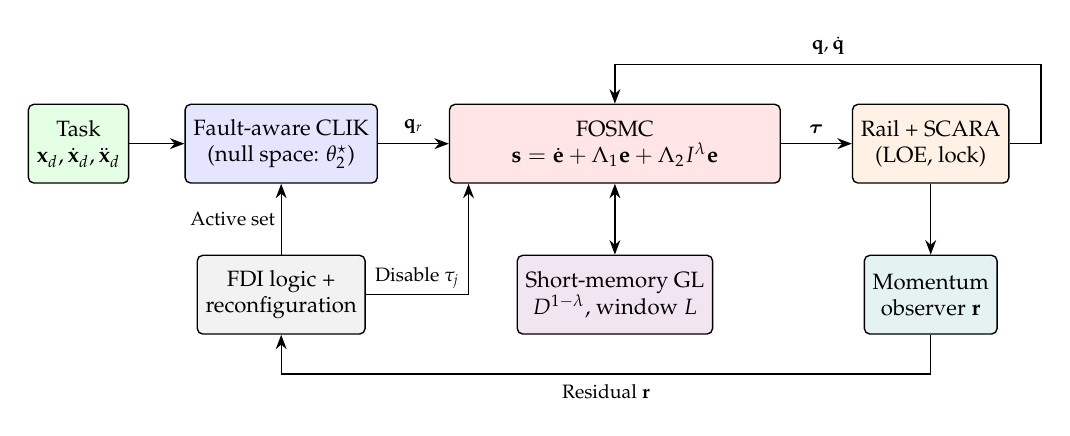
\begin{tikzpicture}[font=\footnotesize, >=Stealth, line width=0.5pt,
  blk/.style={draw, rounded corners=2pt, align=center, minimum height=10mm, inner sep=3pt, fill=#1!10}, blk/.default=gray,
  lab/.style={font=\scriptsize, fill=white, inner sep=1pt}]
% ---- forward path (top row)
\node[blk=green] (task) {Task\\$\mathbf{x}_d,\dot{\mathbf{x}}_d,\ddot{\mathbf{x}}_d$};
\node[blk=blue, right=7mm of task] (clik) {Fault-aware CLIK\\(null space: $\theta_2^\star$)};
\node[blk=red, right=9mm of clik, minimum width=42mm] (ctrl) {FOSMC\\ $\mathbf{s}=\dot{\mathbf{e}}+\Lambda_1\mathbf{e}+\Lambda_2 I^{\lambda}\mathbf{e}$};
\node[blk=orange, right=9mm of ctrl] (rob) {Rail + SCARA\\(LOE, lock)};
% ---- second row
\node[blk=violet, below=9mm of ctrl, minimum width=24mm] (gl) {Short-memory GL\\ $D^{1-\lambda}$, window $L$};
\node[blk=teal, below=9mm of rob] (obs) {Momentum\\observer $\mathbf{r}$};
\node[blk=gray, below=9mm of clik] (fdi) {FDI logic +\\ reconfiguration};
% ---- signals
\draw[->] (task) -- (clik);
\draw[->] (clik) -- node[above, font=\scriptsize]{$\mathbf{q}_r$} (ctrl);
\draw[->] (ctrl) -- node[above, font=\scriptsize]{$\boldsymbol{\tau}$} (rob);
\draw[->] (rob.east) -- ++(4mm,0) coordinate (fb) |- ($(ctrl.north)+(0,5mm)$) node[pos=0.75, above, font=\scriptsize]{$\mathbf{q},\dot{\mathbf{q}}$} -- (ctrl.north);
\draw[<->] (ctrl) -- (gl);
\draw[->] (rob) -- (obs);
% Residual: below the second row, so that it never crosses the GL block
\draw[->] (obs.south) -- ++(0,-5mm) -| node[pos=0.25, below, font=\scriptsize]{Residual $\mathbf{r}$} (fdi.south);
\draw[->] (fdi) -- node[lab, left=1pt]{Active set} (clik);
% Disable command: leaves FDI to the right, rises in the gap left of the GL block
\draw[->] (fdi.east) -- ($(fdi.east -| ctrl.south west)+(2.5mm,0)$) node[lab, pos=0.5, above=1pt]{Disable $\tau_j$} -- ($(ctrl.south west)+(2.5mm,0)$);
\end{tikzpicture}
\end{document}
